\chapter{Parte 2}
\label{cap:p2}

\section{Análise Problema}

Na Parte I o problema tratava de achar o caminho mais longo de uma rede. Nesta
parte, partindo da mesma rede, pretende-se descobrir o tempo em que cada
atividade é iniciada, sabendo que todas as atividades são realizadas.

\section{Modelo}

\subsection{Parâmetros}

À semelhança da Parte I, também aqui os parâmetros do problema são a duração de
cada atividade e as suas precedências.

\subsection{Variáveis de decisão}

As variáveis de decisão correspondem ao tempo em que cada atividade é iniciada.
Assim, a cada atividade está associada uma variável de decisão. Relativamente ao
nome, a opção tomada foi a de considerar $T_{i}$ como o tempo de início da
atividade $i$ (em unidades de tempo arbitrárias), em que $i$ corresponde ao número da atividade. Uma vez que apenas se pretende conhecer os tempos de início de cada atividade, estas são as únicas variáveis deste modelo. 

\subsection{Função Objetivo}

Neste modelo, quer-se minimizar o tempo de execução total do projeto. Isso
corresponde a dizer que queremos que a atividade final seja iniciada o mais cedo
possível. A atividade final é na verdade ``fictícia'', pois não corresponde
a uma atividade que tenha de ser efetivamente realizada. No entanto para efeitos
de modelação, é útil considerá-la, assumindo que é realizada após todas as
outras da rede terem terminado e que tem duração de 0 unidades de tempo. Nestas
condições, o tempo inicial da atividade final indica a duração do
projeto.

Uma vez que a variável $T_{fim}$ indica a duração do projeto, a função
objetivo fica simplesmente:

\begin{displaymath} \min~z = T_{fim} \end{displaymath}

\subsection{Restrições}

Com as restrições pretende-se indicar o espaço de possíveis soluções. Sabe-se que uma
atividade não pode começar sem que as que lhe precedem tenham terminado.
Qualquer solução que obedeça a este princípio é uma solução admissível para
o problema. Para escrever as restrições é por isso necessário saber quando uma atividade termina. Ora, sabendo que as nossas variáveis de decisão indicam o tempo em que
cada atividade se inicia e que temos a duração das mesmas como parâmetro do modelo, podemos dizer que o tempo final de uma atividade corresponde a somar o seu tempo de início com a sua duração. Ou seja:

\begin{displaymath} Tf_{i} = T_{i} + D_{i} \end{displaymath}

Onde:

\begin{itemize} \item[$Tf_{i}$] Tempo em que a atividade $i$ termina
		\item[$T_{i}$] Tempo em que a atividade i começa (variável de decisão)
		\item[$D_{i}$] Duração da atividade $i$ \end{itemize}

Dizer que uma atividade não pode começar sem que as que lhe precedem tenham
terminado é o mesmo que dizer que o tempo inicial da atividade tem que ser maior
que o tempo final de todas as atividades que lhe precedem. Assumindo que se tem
uma atividade $j$ que precede uma atividade $i$, podemos escrever que:

\begin{displaymath} T_{i} \geq T_{j} + D_{j} \end{displaymath}

O modelo terá por isso uma restrição deste tipo por cada nodo e por cada
atividade precedente ao nodo. Ou seja, um nó que tenha apenas 1 precedência,
apenas originará uma restrição, enquanto que se o nodo tiver por exemplo
3 precedências, dará origem a 3 restrições --- uma restrição para cada precedência
do nodo. As restrições completas podem ser consultadas na secção \ref{p2:sec:ficheiro_input}

Visto que os tempos não podem ser negativos, neste modelo tem-se ainda
restrições de não-negatividade:

\begin{displaymath} T_{i} \geq 0, \forall i_{\in\{ini, 0, 1, 3,
	4,5,6,7,9,10,11,fim\}} \end{displaymath}


\section{Ficheiro \emph{input}}
\label{p2:sec:ficheiro_input}
O ficheiro de \emph{input} é constituído pela função objetivo e restrições, detalhadas
em secções anteriores.

\begin{verbatim}

=== FUNCAO objetivo ===

min: Tfim;


=== RESTRICOES ===

//Nodo Inicial
Tini >= 0 + 0;

//Nodo 0
T0 >= Tini + 0;

//Nodo 1
T1 >= T0 + 4;

//Nodo 3
T3 >= T1 + 6;
T3 >= T5 + 4;
T3 >= T4 + 9;

//Nodo 4
T4 >= T0 + 4;
T4 >= T7 + 6;

//Nodo 5
T5 >= T4 + 9;
T5 >= T7 + 6;
T5 >= T10 + 8;

//Nodo 6
T6 >= Tini + 0;

//Nodo 7
T7 >= T6 + 5;

//Nodo 9
T9 >= T7 + 6;
T9 >= T11 + 7;
T9 >= T10 + 8;

//Nodo 10
T10 >= T6 + 5;

//Nodo 11
T11 >= T10 + 8;

//Nodo final
Tfim >= T3 + 2;
Tfim >= T5 + 4;
Tfim >= T9 + 2;

\end{verbatim}



\newpage
\section{\emph{Output} produzido pelo \texttt{lp\_solve}}

O output apresentado a seguir foi obtido por \emph{copy-paste} direto resultante da execução do \emph{lp\_solve} num sistema linux para o ficheiro de input apresentado anteriormente:

\begin{verbatim} 

Value of objective function: 26

Actual values of the variables:
Tfim                           26
Tini                            0
T0                              0
T1                              4
T3                             24
T5                             20
T4                             11
T7                              5
T10                             5
T6                              0
T9                             20
T11                            13

Actual values of the constraints:
R1                              0
R2                              4
R3                             20
R4                              4
R5                             13
R6                             11
R7                              6
R8                              9
R9                             15
R10                            15
R11                             0
R12                             5
R13                            15
R14                             7
R15                            15
R16                             5
R17                             8
R18                             2
R19                             6
R20                             6



\end{verbatim}

\section{Resultado}

O resultado obtido indica uma duração total do projeto de 26 unidades de tempo. Os tempos iniciais de cada atividade representados graficamente podem ser vistos na figura \ref{p2:fig:tempos_inicio} :

\begin{figure}[<+htpb+>] \centering
	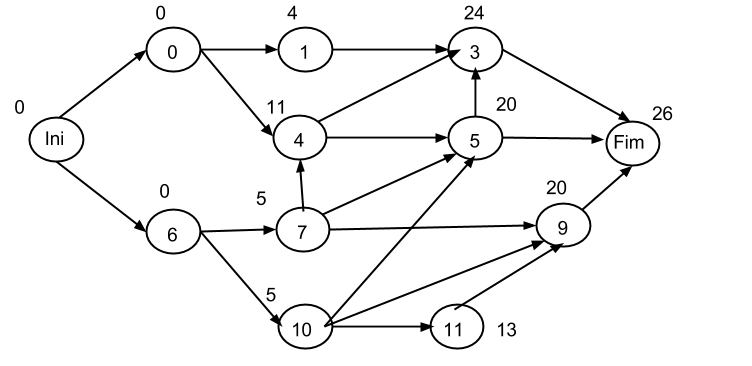
\includegraphics[scale=0.5]{./img/p2_tempos_inicio} \caption{Grafo com
	tempo de início de cada atividade (em unidades de tempo arbitrárias)}
\label{p2:fig:tempos_inicio}
 \end{figure}

O Diagrama de Gantt correspondente pode ser visto na figura \ref{p2:fig:diagrama_gantt_caminho_crit}:

\begin{figure}[<+htpb+>] \centering
	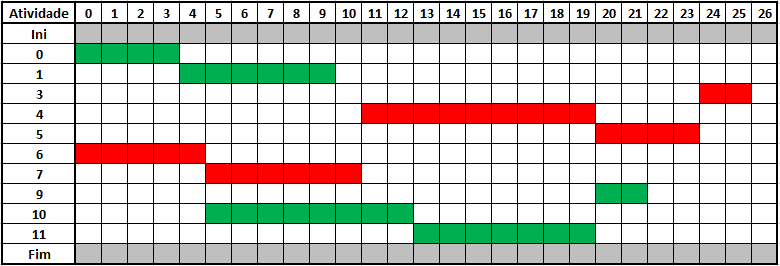
\includegraphics[width=\textwidth]{./img/p2_diagrama_gantt_caminho_crit}
	\caption{Diagrama de \emph{Gantt} com indicação do caminho crítico a vermelho}
\label{p2:fig:diagrama_gantt_caminho_crit} \end{figure}

Visto serem atividades fictícias de duração nula, representam-se atividades
iniciais e finais a cinzento. As barras a vermelho indicam o caminho crítico,
enquanto que as barras a verde representam atividades não pertencentes ao
caminho crítico.

\section{Validação do modelo}

Para validar os resultados, tanto na função objetivo como nas restrições,
substituímos os valores das variáveis de decisão pelo valor que estas tomam na
solução que o \texttt{lp\_solve} indica como ótima. A ideia é verificar que os valores das
variáveis de decisão obtidos confirmam o valor da função objetivo obedecendo
a todas as restrições.

Para evitar ao máximo o erro humano, a substituição de variáveis foi feita
recorrendo a ferramentas que auxiliaram a substituição automática das variáveis
pelo seu valor.

\subsection{Variáveis de decisão}

No resultado obtido, todas as variáveis tomam um valor maior ou igual a 0, tal
como seria de esperar.

\subsection{Função objetivo}

Neste modelo a função objetivo consiste apenas no valor de uma variável,
$T_{fim}$, que vale 26 unidades de tempo na solução ótima. Por motivos que não fazem parte do
âmbito deste trabalho, o valor esperado para a duração mínima
do projeto deverá ser o mesmo valor de duração encontrado no caminho crítico da
Parte I. O valor obtido corresponde de facto ao esperado, uma vez que a duração do
caminho crítico obtido na Parte I foi também igual a 26 unidades de tempo.


\subsection{Restrições}


\begin{verbatim} 

//Nodo Inicial
Tini >= 0 + 0;
0 >= 0 + 0;

//Nodo 0
T0 >= Tini + 0; 
0 >= 0 + 0;

//Nodo 1
T1 >= T0 + 4; 
4 >= 0 + 4;

//Nodo 3
T3 >= T1 + 6; 
24 >= 4 + 6;

T3 >= T5 + 4; 
24 >= 20 + 4;

T3 >= T4 + 9; 
24 >= 11 + 9;

//Nodo 4
T4 >= T0 + 4; 
11 >= 0 + 4;

T4 >= T7 + 6; 
11 >= 5 + 6;

//Nodo 5
T5 >= T4 + 9; 
20 >= 11 + 9;

T5 >= T7 + 6; 
20 >= 5 + 6;

T5 >= T10 + 8; 
20 >= 5 + 8;

//Nodo 6
T6 >= Tini + 0; 
0 >= 0 + 0;

//Nodo 7
T7 >= T6 + 5; 
5 >= 0 + 5;

//Nodo 9
T9 >= T7 + 6; 
20 >= 5 + 6;

T9 >= T11 + 7; 
20 >= 13 + 7;

T9 >= T10 + 8; 
20 >= 5 + 8;

//Nodo 10
T10 >= T6 + 5; 
5 >= 0 + 5;

//Nodo 11
T11 >= T10 + 8; 
13 >= 5 + 8;

//Nodo final
Tfim >= T3 + 2; 
26 >= 24 + 2;

Tfim >= T5 + 4; 
26 >= 20 + 4;

Tfim >= T9 + 2; 
26 >= 20 + 2;

\end{verbatim}

Assim conclui-se que todas as restrições são respeitadas.

\section{Atividade no caminho crítico}

Considere-se a atividade 7, que faz parte do caminho crítico. Por análise do
resultado do modelo verifica-se que esta atividade deve começar em $T = 5~u.t$. Como
é facilmente visível no Diagrama de \emph{Gantt} apresentado na figura \ref{p2:fig:diagrama_gantt_caminho_crit},
caso a atividade comece um pouco mais tarde, irá atrasar o começo da atividade
que lhe sucede, neste caso a atividade 4. Se a atividade 4 começar mais tarde,
por sua vez vai atrasar o início da atividade 5, que lhe sucede. Seguindo
a mesma lógica a atividade 5 começando mais tarde atrasa o início da atividade
3. Visto a atividade 3 ser a última atividade a ser realizada, tal atraso implica um atraso no tempo de execução total do projeto.

Obtém-se resultados semelhantes caso sejam provocados atrasos em outras atividades pertencentes ao caminho crítico. Com isto mostra-se o impacto que um atraso na execução de uma atividade no caminho crítico tem no projeto total.

\section{Atividade fora do caminho crítico}

Considere-se a atividade 1, não pertencente ao caminho crítico. De acordo com os
resultados do modelo, esta atividade deve ter início em $T_{1} = 4~u.t$. Por análise do Diagrama de Gantt da figura \ref{p2:fig:diagrama_gantt_caminho_crit}, verifica-se que no entanto, esta pode começar um pouco mais tarde. A atividade 1 apenas
é sucedida pela atividade 3, sendo que a atividade 3 apenas deve ter início em
$T_{3} = 24~u.t$. Como restrição do modelo, sabemos que a soma do tempo de início de
uma atividade com a sua duração não deve ser maior que o tempo de início de
qualquer atividade sucessora. No limite, uma atividade acaba imediatamente antes
de uma sua sucessora começar. Traduzindo esse facto em termos matemáticos, no
caso da atividade 1 temos que:

\begin{displaymath} T_{1} + D_{1} = T_{3} \end{displaymath}

Onde:

\begin{itemize} \item[$T_{1}$] Tempo de início da atividade 1 \item[$D_{1}$]
		Duração da atividade 1 \item[$T_{3}$] Tempo de início da atividade
			3 \end{itemize}

Resolvendo a equação em ordem a $T_{1}$ temos:

\begin{displaymath}
T_{1} + 6 = 24~u.t \Leftrightarrow T_{1} = 18~u.t
\end{displaymath}

Isto significa que no limite, a atividade 1 pode começar em $T_{1} = 18~u.t$ sem que
haja atrasos no projeto, embora os resultados do modelo sugiram um tempo inicial $T_{1} = 4~u.t$.

A situação descrita aqui para a atividade 1 acontece também com outras atividades que não pertencem ao caminho crítico. A conclusão que se tira é que pode haver atrasos (dentro de certos limites) nas atividades que não pertencem ao caminho crítico sem que isso tenha influência no tempo total do projeto.
